\chapter{Thermische Geschichte, letzte Streuung und die Ursuppe}

\lectureoverview{Die Expansionsgeschichte des Universums ist zugleich eine thermische Geschichte. Wir beginnen damit, die Temperatur über das Gleichgewicht und das Gleichgewicht über Streuung zu definieren. Ein Photonengas nimmt das Planck-Spektrum an, solange freie Ladungsträger es im thermischen Gleichgewicht halten; wenn sich Elektronen an Protonen binden, entkoppelt die Strahlung, behält aber ihre Schwarzkörperform bei, während sich jede Wellenlänge mit dem Skalenfaktor vergrößert. Das enorme Verhältnis von Photonen zu Materie erklärt dann, warum die Rekombination bei einer Temperatur weit unterhalb der Wasserstoff-Ionisationstemperatur stattfindet. Gehen wir weiter zurück, gelangen wir zur letzten Streuung, zur Materie--Strahlungs-Gleichheit, zum Gleichgewicht von Elektron--Positron-Paaren und schließlich zum kleinen Materie--Antimaterie-Überschuss, der die Annihilation überdauert.}

\section{Von der Modellanpassung zur thermischen Geschichte}

Ein kosmologisches Modell wird mindestens durch den zeitlichen Verlauf des Skalenfaktors und eine räumliche Geometrie festgelegt,
\begin{equation}
a(t),
\qquad
k\in\{+1,0,-1\}.
\end{equation}
Die praktische Methode besteht darin, das Modell auszuwählen, seine Vorhersagen zu berechnen, diese mit Daten zu vergleichen und die Parameter anzupassen. Die Schlussfolgerung direkt aus den Daten rückwärts zu ziehen, ist möglich, aber oft weniger transparent.

Die Krümmung lässt sich anhand vergleichsweise naher Quellen nur schwer bestimmen. So wie die Erdkrümmung über eine kurze Strecke auf der Erdoberfläche nur eine kleine Korrektur darstellt, ist auch die räumliche Krümmung ein schwacher Effekt, wenn die kosmologische Vergleichsstrecke nicht groß genug ist. Das ist zugleich ein Nachteil und ein Vorteil: Gewöhnliche Quellensurveys bestimmen \(k\) nicht genau, doch eine mäßige Unsicherheit in \(k\) verhindert keine brauchbare Rekonstruktion der Expansionsgeschichte.

Zwei Klassen von Observablen tragen einen großen Teil dazu bei. Standardkerzen liefern die Helligkeit als Funktion der Rotverschiebung, während Quellensurveys die Anzahl der Objekte in einem Rotverschiebungsintervall angeben. Die resultierenden Anpassungen sprechen für eine Expansionsgeschichte mit einem erheblichen Beitrag der Vakuumenergie. Präzise Informationen über die Krümmung erfordern den viel größeren geometrischen Hebelarm, den die kosmische Mikrowellenhintergrundstrahlung bietet.

Wir stellen nun eine andere Frage. Statt nur zu fragen, wie sich \(a(t)\) entwickelt, fragen wir, wie sich die Temperatur des Universums entwickelt. Diese Frage beginnt mit einer grundsätzlicheren: Unter welchen Bedingungen hat ein System überhaupt eine Temperatur?

\section{Wann ein Universum eine Temperatur hat}

Die Temperatur ist eine Eigenschaft des thermischen Gleichgewichts. Ein Teilchensystem nähert sich durch Stöße dem Gleichgewicht, und diese Stöße müssen schneller ablaufen, als sich die makroskopische Umgebung verändert. In einem expandierenden Universum ist der sinnvolle Vergleich
\begin{equation}
\tau_{\rm scatt}\ll H^{-1},
\label{eq:c07-equilibrium-condition}
\end{equation}
Dabei ist \(\tau_{\rm scatt}\) eine charakteristische Streuungszeit und \(H^{-1}\) die Expansionszeit. Gilt diese Ungleichung nicht, verändert sich das Universum, bevor Stöße das Gleichgewicht wiederherstellen können.

Betrachten wir einen perfekt reflektierenden Kasten. Wir richten einen Laserpuls hinein, schließen die Öffnung und nehmen an, dass sich darin ausschließlich Photonen befinden. Der Puls prallt unbegrenzt hin und her, doch gewöhnliche Photonen niedriger Energie streuen nur außerordentlich schwach aneinander. Die Reflexion allein verteilt ihre Energie nicht zu einem thermischen Spektrum um. Ein Photonengas wird also nicht allein dadurch thermisch, dass es eingeschlossen ist.

Freie geladene Teilchen verändern die Situation. Eine elektromagnetische Welle beschleunigt ein Elektron; die beschleunigte Ladung strahlt erneut ab, sodass Photonen wirksam gestreut werden. Bei genügend vielen freien Elektronen und Protonen verteilt wiederholte Streuung die Energie auf alle drei Teilchensorten, bis sie eine gemeinsame thermische Mischung mit einheitlicher Temperatur bilden.

Auf großen Skalen ist das Universum elektrisch neutral. In der einfachsten Zählweise gilt
\begin{equation}
n_{e^-}=n_p,
\label{eq:c07-neutrality}
\end{equation}
weil die Beträge der Elektronen- und Protonenladung gleich und ihre Vorzeichen entgegengesetzt sind. Diese Gleichung besagt, dass das Universum neutral ist; sie erklärt weder, warum die Ladung neutral ist, noch warum die beiden Ladungsbeträge übereinstimmen. Das sind tiefer liegende Tatsachen der Teilchenphysik.

Der Unterschied zwischen einem Plasma und einem neutralen Gas ist entscheidend. Freie Elektronen streuen Strahlung wirksam. Sobald sich Elektronen an Protonen binden und neutralen Wasserstoff bilden, heben sich die dominierenden elektrischen Felder über große Entfernungen auf, und die Streuung wird deutlich schwächer. Bei der geringen Dichte des heutigen Universums kann neutrale Materie die Hintergrundphotonen innerhalb eines kosmischen Alters nicht ins Gleichgewicht bringen.

Bei hinreichend hoher Temperatur ionisieren energiereiche Stöße Wasserstoff immer wieder und halten einen beträchtlichen Anteil freier Ladungsträger aufrecht. Elektronen, Protonen und Photonen haben dann dieselbe Temperatur. Kühlt das System ab, bleiben Atome bestehen, die Dichte freier Elektronen bricht ein, und das gemeinsame Gleichgewicht geht verloren. Die Materie und die Strahlung haben danach nicht notwendigerweise dieselbe Temperatur.

\begin{classroomqa}
\audiencequestion{Wenn die Mikrowellenhintergrundstrahlung eine Temperatur von etwa \(3\,\mathrm{K}\) hat, ist das dann die Temperatur des gesamten Universums heute?}
\lecturerresponse{Nein. Das Photonenspektrum lässt sich durch eine Schwarzkörpertemperatur beschreiben, aber die heutige Materie steht mit diesen Photonen nicht im Gleichgewicht. Verschiedene Komponenten haben unterschiedliche kinetische oder effektive Temperaturen, sodass es heute keine einzige globale thermodynamische Temperatur gibt.}
\end{classroomqa}

\section{Thermische Strahlung und der quantenmechanische Umschlag}

Ein Strahlungsfeld im Gleichgewicht enthält ein Spektrum von Wellenlängen und Frequenzen, die durch
\begin{equation}
\nu\lambda=c.
\end{equation}
zusammenhängen. Damit die Strahldichte nicht mit der Energiedichte verwechselt wird, bezeichne \(u_\nu(T)\) die Energie pro Volumeneinheit und Frequenzintervall:
\begin{equation}
dE=u_\nu(T)\,dV\,d\nu.
\label{eq:c07-spectral-density}
\end{equation}
Damit hat \(u_\nu\) die Dimension Energie dividiert durch Volumen und Frequenz.

Die Temperatur selbst ist eine Energieskala. Historische Temperatureinheiten verschleiern diese Tatsache; die Umrechnung erfolgt mit der Boltzmann-Konstanten:
\begin{equation}
E_{\rm thermal}\sim k_B T.
\end{equation}
Man kann in natürlichen Einheiten \(k_B=1\) setzen, doch wenn man sie beibehält, bleiben Kelvin und Energie sichtbar voneinander unterschieden.

Vor der Quantenmechanik ergibt die Dimensionsanalyse mit \(k_BT\), \(\nu\) und \(c\) die spektrale Rayleigh--Jeans-Energiedichte,
\begin{equation}
u_\nu^{\rm RJ}(T)=\frac{8\pi\nu^2}{c^3}k_BT.
\label{eq:c07-rayleigh-jeans}
\end{equation}
Der Zahlenfaktor hängt davon ab, wie die elektromagnetischen Moden gezählt werden; entscheidend ist jedoch das klassische Verhalten \(u_\nu\propto T\nu^2\). Die Energiedichte wächst mit zunehmender Frequenz unbegrenzt und sagt daher voraus:
\begin{equation}
\int_0^\infty u_\nu^{\rm RJ}\,d\nu=\infty.
\end{equation}
Dieses unmögliche Ergebnis ist die Ultraviolett-Katastrophe. Das gemessene Spektrum steigt stattdessen zunächst an, erreicht einen Umschlagpunkt und fällt dann so stark ab, dass die Gesamtenergie endlich bleibt.

Das Plancksche Wirkungsquantum führt die fehlende Quantenskala ein. Für die in Gleichung~\eqref{eq:c07-spectral-density} definierte spektrale Energiedichte lautet das Plancksche Gesetz:
\begin{equation}
u_\nu(T)
=
\frac{8\pi h\nu^3}{c^3}
\frac{1}{e^{h\nu/(k_BT)}-1}.
\label{eq:c07-planck}
\end{equation}
Der Exponent hängt vom dimensionslosen Verhältnis
\begin{equation}
x=\frac{h\nu}{k_BT},
\end{equation}
ab, denn \(E_\gamma=h\nu\) und \(k_BT\) sind beides Energien.

Bei niedriger Frequenz gilt \(x\ll1\), und
\begin{equation}
e^x-1=x+O(x^2).
\end{equation}
Einsetzen in Gleichung~\eqref{eq:c07-planck} ergibt
\begin{align}
u_\nu(T)
&\simeq
\frac{8\pi h\nu^3}{c^3}
\frac{k_BT}{h\nu}
\\
&=
\frac{8\pi\nu^2}{c^3}k_BT,
\end{align}
Damit wird die klassische Physik in ihrem gültigen Niederfrequenzbereich wiedergewonnen. Bei hoher Frequenz gilt \(x\gg1\); dann dominiert der Exponentialterm und unterdrückt das Spektrum. Der Übergang findet statt bei
\begin{equation}
\frac{h\nu}{k_BT}\sim1.
\label{eq:c07-crossover}
\end{equation}
An diesem Punkt wird der klassische Anstieg durch den quantenmechanischen Umschlag abgelöst.

\begin{figure}[htbp]
\centering
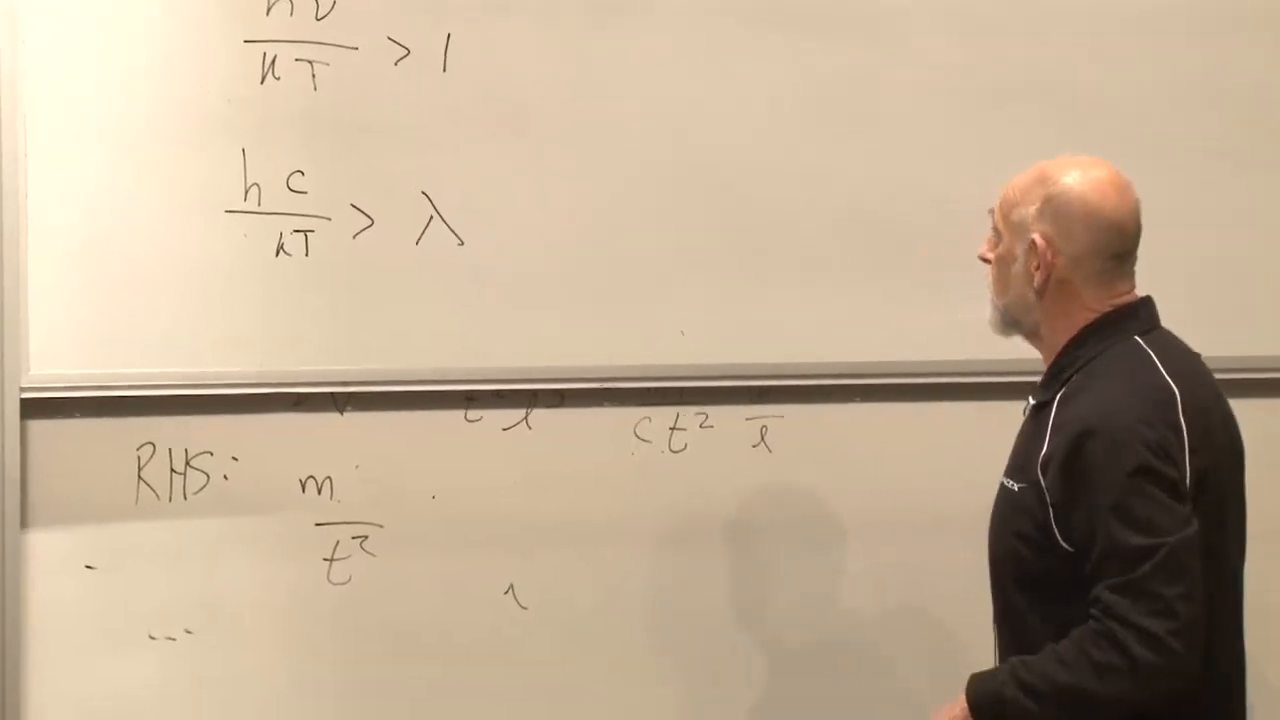
\includegraphics[width=0.82\textwidth]{lecture_07_figure_02.png}
\caption{Der thermische Übergang auf der Tafel. Der oben abgeschnittene Ausdruck lautet \(h\nu/(kT)>1\), und der klar erkennbare untere Ausdruck lautet \(hc/(kT)>\lambda\). Schwache Reste auf der unteren Tafel werden nicht als Beleg für eine Gleichung verwendet.}
\label{fig:c07-thermal-board}
\lectureframe{00:44:42.840}
\end{figure}

Mit \(\nu=c/\lambda\) legt der Übergangspunkt eine thermische Wellenlänge in der Größenordnung
\begin{equation}
\boxed{\lambda_{\rm th}\sim\frac{hc}{k_BT}}.
\label{eq:c07-thermal-wavelength}
\end{equation}
fest. Kürzere Wellenlängen liegen im exponentiell unterdrückten Ausläufer; der größte Teil der Leistung entfällt auf Wellenlängen dieser Größenordnung, bis auf einen Zahlenfaktor, der davon abhängt, ob das Spektrum pro Frequenz- oder pro Wellenlängeneinheit dargestellt wird.

\begin{classroomqa}
\audiencequestion{Hat Planck das Spektrum aus dem hier verwendeten Modell eines Elektron--Protonenplasmas hergeleitet?}
\lecturerresponse{Nein. Er kombinierte empirische Spektralinformationen mit dem Wienschen Verschiebungsgesetz, das bereits zeigte, dass die Wellenlänge des Maximums umgekehrt proportional zur Temperatur ist. Diese Skalierung ließ eine neue Konstante \(h\) erkennen. Planck verknüpfte das Ergebnis mit Oszillatoren in den materiellen Wänden; die vollständige quantenmechanische Deutung des Strahlungsfeldes kam später hinzu. \lecturetimestamp{00:37:06--00:39:25}}
\end{classroomqa}

\begin{classroomqa}
\audiencequestion{Warum schien die Dimensionsprüfung eine Potenz von \(c\) zu wenig zu ergeben?}
\lecturerresponse{Die zunächst als Intensität bezeichnete Größe war als Energie pro Volumen und Frequenz definiert, während die bekannte Formel mit \(2h\nu^3/c^2\) die spektrale Strahldichte pro Fläche und Raumwinkel angibt. Die spektrale Energiedichte enthält \(c^{-3}\) und einen Winkelterm, wie in Gleichung~\eqref{eq:c07-planck}. Die Korrektur ändert die Normierungskonvention, nicht das dimensionslose Verhältnis \(h\nu/(k_BT)\) oder die thermische Wellenlänge. \lecturetimestamp{00:39:33--00:44:51}}
\end{classroomqa}

Abgesehen von der Normierung hat das Planck-Spektrum eine universelle Form. Gleichung~\eqref{eq:c07-planck} lässt sich schreiben als
\begin{equation}
u_\nu(T)=T^3\,F\!\left(\frac{\nu}{T}\right),
\label{eq:c07-scaling-form}
\end{equation}
wobei Konstanten in \(F\) aufgenommen sind. Eine Erhöhung von \(T\) skaliert die Frequenzachse und die Gesamthöhe; dieselbe dimensionslose Kurve erscheint wieder. In der Darstellung nach Wellenlänge verschiebt eine Temperaturerhöhung das Spektrum zu kürzeren Wellenlängen.

\begin{figure}[htbp]
\centering
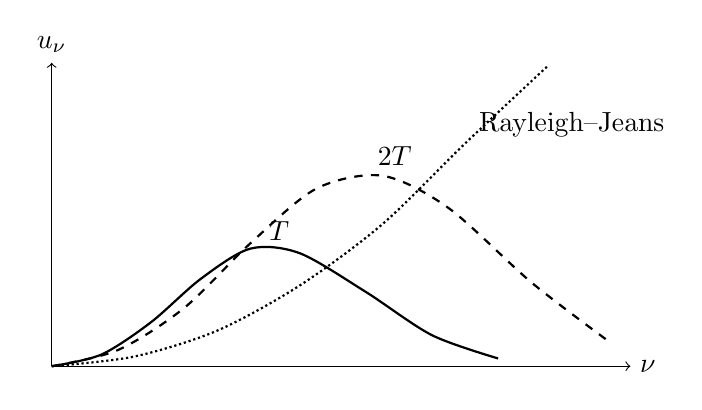
\begin{tikzpicture}[x=1.05cm,y=0.82cm]
\draw[->] (0,0)--(7.0,0) node[right] {\(\nu\)};
\draw[->] (0,0)--(0,4.7) node[above] {\(u_\nu\)};
\draw[densely dotted,thick] plot[smooth] coordinates
  {(0,0) (1,0.15) (2,0.55) (3,1.25) (4,2.20) (5,3.45) (6,4.65)};
\draw[thick] plot[smooth] coordinates
  {(0,0) (0.6,0.18) (1.2,0.68) (1.8,1.35) (2.4,1.82) (3.0,1.75) (3.8,1.15) (4.6,0.48) (5.4,0.12)};
\draw[thick,dashed] plot[smooth] coordinates
  {(0,0) (0.8,0.25) (1.6,0.90) (2.4,1.90) (3.2,2.75) (4.0,2.95) (4.8,2.45) (5.8,1.30) (6.7,0.42)};
\node[anchor=west] at (5.05,3.75) {Rayleigh--Jeans};
\node at (2.75,2.10) {\(T\)};
\node at (4.15,3.25) {\(2T\)};
\end{tikzpicture}
\caption{Das klassische Spektrum steigt unbegrenzt an, während die Planck-Spektren einen Umschlag zeigen. Mit steigender Temperatur verschiebt sich die charakteristische Frequenz nach oben, und die dimensionslose Form bleibt erhalten.}
\label{fig:c07-planck-redraw}
\end{figure}

Der mit Abstand größte Teil der Photonen im heutigen Universum gehört zur Mikrowellenhintergrundstrahlung und hat eine charakteristische Wellenlänge in der Größenordnung eines Millimeters. Gleichung~\eqref{eq:c07-thermal-wavelength} ordnet dieser Wellenlänge eine Temperatur von einigen Kelvin zu, die hier der Einfachheit halber auf \(3\,\mathrm{K}\) gerundet wird. Eine Wellenlänge allein würde nur eine grobe Zuordnung erlauben. Der stärkere Beleg besteht darin, dass Messungen bei vielen Frequenzen mit sehr hoher Genauigkeit der vollständigen Schwarzkörperkurve folgen.

\begin{classroomqa}
\audiencequestion{Wie viel Raum nimmt ein einzelnes Photon der Mikrowellenhintergrundstrahlung ein?}
\lecturerresponse{Ein Photon hat keine universelle, scharf begrenzte Größe. Es kann als Wellenpaket präpariert werden, dessen räumliche Ausdehnung vom Zustand abhängt; seine Wellenlänge legt dabei die Skala seiner Schwingung fest. Bei der thermischen Hintergrundstrahlung liegen sowohl die charakteristische Wellenlänge als auch eine natürliche Skala des Wellenpakets in der Größenordnung eines Millimeters. Beides sollte jedoch nicht mit dem Radius eines kleinen klassischen Objekts verwechselt werden. \lecturetimestamp{00:57:16--00:59:05}}
\end{classroomqa}

\section{Die Expansion bewahrt die Schwarzkörperform}

Wir beginnen mit einem heißen Kasten, der ionisierten Wasserstoff und Strahlung im Gleichgewicht enthält. Während sich der Kasten ausdehnt, verrichtet sein Inhalt Arbeit, die Energiedichte sinkt und die Temperatur fällt. Schließlich bleiben Elektronen und Protonen als neutrale Atome gebunden. Die Bildung von Atomen heißt \emph{Rekombination}; der Verlust wirksamer Streuung zwischen Photonen und Materie heißt --\emph{Entkopplung}. Die beiden Prozesse hängen eng zusammen, bezeichnen aber unterschiedliche physikalische Ereignisse.

Nach der Entkopplung haben Materie und Strahlung keine gemeinsame Temperatur mehr. Dennoch behält das Photonenspektrum seine Planck-Form. Jede sich frei ausbreitende Wellenlänge wird um denselben Expansionsfaktor gestreckt:
\begin{equation}
\lambda\propto a,
\qquad
\nu\propto a^{-1}.
\end{equation}
Da die Planck-Kurve von \(\nu/T\) abhängt, entspricht diese gleichmäßige Rotverschiebung einer Strahlungstemperatur von
\begin{equation}
\boxed{T_\gamma\propto a^{-1}.}
\label{eq:c07-temperature-scaling}
\end{equation}
Die Expansion bewahrt also die Form, auch wenn Stöße sie nicht fortlaufend neu herstellen. Die Materie folgt anschließend ihrer eigenen thermischen Geschichte.

Die beobachtete Mikrowellenhintergrundstrahlung ist somit eine fossile Gleichgewichtsverteilung. Ihre Schwarzkörperform entstand, als freie Ladungsträger wirksam streuten, und wurde danach durch die gleichmäßige kosmologische Rotverschiebung weitergetragen. Sternenlicht, Gammastrahlung und andere spätere Quellen gibt es zwar, doch sind sie zahlenmäßig unbedeutend gegenüber der fossilen Photonenpopulation und haben erkennbare astrophysikalische Ursprünge.

\begin{classroomqa}
\audiencequestion{Wie kann Strahlung Schwarzkörperstrahlung bleiben, nachdem sie nicht mehr mit Materie im Gleichgewicht steht?}
\lecturerresponse{Stöße sind nötig, um das Gleichgewichtsspektrum zu erzeugen, nicht aber, um es bei vollkommen gleichmäßiger Expansion zu bewahren. Werden alle Wellenlängen mit demselben Faktor multipliziert, geht ein Planck-Spektrum in ein anderes mit niedrigerer Temperatur über. Die Photonen haben dann nicht mehr die Temperatur der Materie, behalten aber ihre eigene Schwarzkörpertemperatur.}
\end{classroomqa}

\section{Warum die Rekombination so spät stattfindet}

Die heutige Wellenlänge und die Wellenlänge bei der Entkopplung hängen zusammen durch
\begin{equation}
\frac{\lambda_0}{\lambda_{\rm dec}}
=
\frac{a_0}{a_{\rm dec}}
=
\frac{T_{\rm dec}}{T_0}.
\label{eq:c07-decoupling-ratio}
\end{equation}
Die Entkopplung ist mathematisch nicht augenblicklich, dauert aber im Vergleich zur anschließenden Geschichte kurz genug, dass man ihr einen charakteristischen Skalenfaktor und eine charakteristische Temperatur zuordnen kann. Hier bezeichnet \(T_0\) die Temperatur der kosmischen Mikrowellenhintergrundstrahlung, nicht die kinetische Temperatur der intergalaktischen Materie.

Die Ionisationsenergie des Wasserstoff-Grundzustands beträgt
\begin{equation}
\chi_H=13.6\,\mathrm{eV}.
\end{equation}
Eine erste Schätzung würde \(k_BT\sim\chi_H\) ansetzen, sodass ein typisches Photon ein Atom ionisieren kann. Diese Schätzung fällt viel zu hoch aus, weil ein thermisches Spektrum einen hochenergetischen Ausläufer enthält und das Universum eine enorme Anzahl von Photonen aufweist.

\begin{figure}[htbp]
\centering
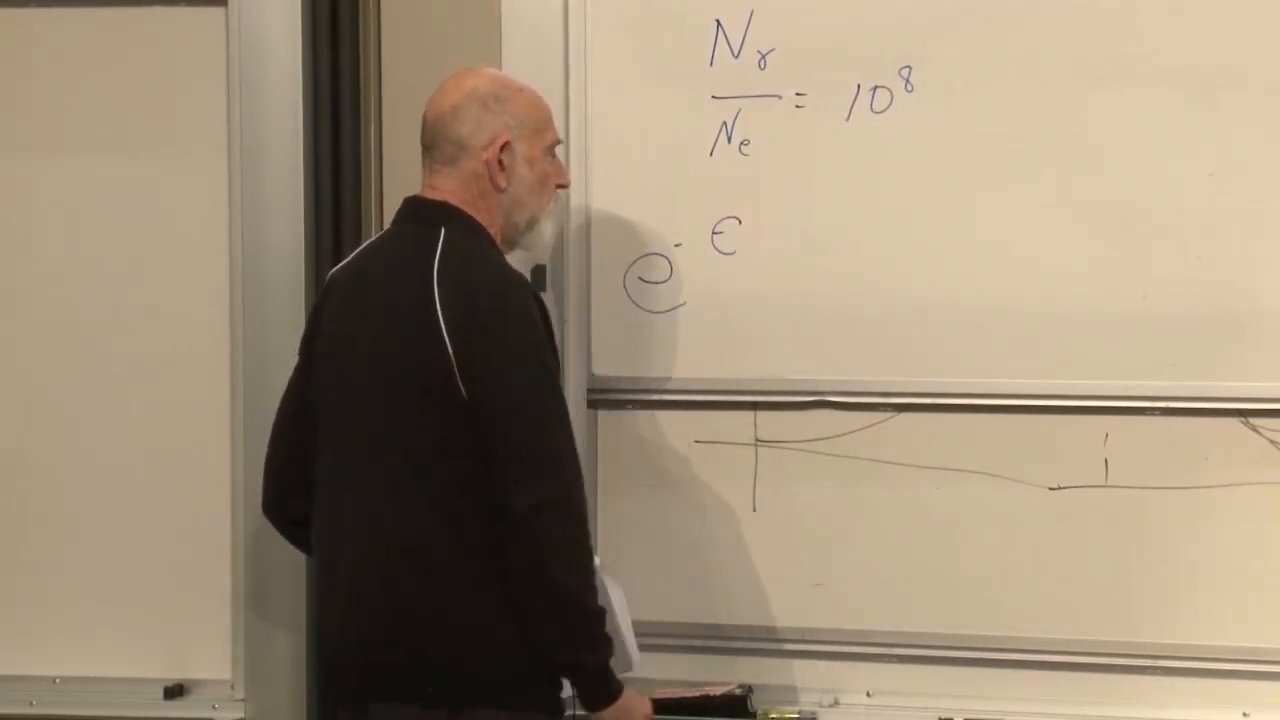
\includegraphics[width=0.82\textwidth]{lecture_07_figure_03.png}
\caption{Auf der Tafel werden das beobachtete Häufigkeitsverhältnis \(N_\gamma/N_e=10^8\) und das Symbol für die Photonenenergie \(\epsilon\) eingeführt. Sichtbar ist nur der Anfang des Exponentialterms; der vollständige Boltzmann-Faktor ergibt sich aus der mündlichen Herleitung.}
\label{fig:c07-boltzmann-board}
\lectureframe{01:06:10.631}
\end{figure}

Das hier verwendete gerundete Häufigkeitsverhältnis lautet
\begin{equation}
\frac{N_\gamma}{N_e}\sim10^8.
\label{eq:c07-photon-electron-ratio}
\end{equation}
Es ergibt sich aus dem Vergleich der gemessenen Photonendichte der kosmischen Mikrowellenhintergrundstrahlung mit dem Bestand gewöhnlicher Materie. Für eine Photonenenergie \(\epsilon\) hat der hochenergetische Ausläufer die Boltzmann-Form
\begin{equation}
P(\epsilon)\propto e^{-\epsilon/(k_BT)}.
\end{equation}
Die Zahl der pro Atom verfügbaren ionisierenden Photonen lässt sich daher abschätzen durch
\begin{equation}
10^8 e^{-\chi_H/(k_BT)}.
\end{equation}
Die Ionisation bleibt wirksam, bis diese Größe auf die Größenordnung eins fällt.

Logarithmieren ergibt
\begin{equation}
\frac{\chi_H}{k_BT}
\sim
\ln 10^8
\simeq18.4,
\end{equation}
oder, mit der hier angestrebten Genauigkeit,
\begin{equation}
k_BT\sim\frac{\chi_H}{20}.
\label{eq:c07-tail-estimate}
\end{equation}
Das charakteristische Photon kann weit unter der Schwelle liegen, denn ein einziges ionisierendes Photon aus dem Ausläufer reicht pro Atom aus.

\begin{classroomqa}
\audiencequestion{Erfasst die Abschätzung des Ausläufers nur Photonen genau an der Schwelle oder alle Photonen oberhalb davon?}
\lecturerresponse{Sie erfasst Photonen an und oberhalb der Schwelle. Da der Ausläufer exponentiell abfällt, kommt der größte Teil dieses Integrals aus Energien in der Nähe von \(\chi_H\). Daher liefert die einfache Exponentialabschätzung die relevante Größenordnung. \lecturetimestamp{01:08:39--01:08:54}}
\end{classroomqa}

\begin{classroomqa}
\audiencequestion{War das Verhältnis \(N_\gamma/N_e\) bei der Entkopplung ebenfalls ungefähr \(10^8\)?}
\lecturerresponse{Bei der hier verwendeten Näherung: ja. Von der Entkopplung zurück bis zu deutlich heißeren Epochen verdünnt die Expansion beide Populationen um denselben Volumenfaktor; außerdem werden von keiner der beiden Teilchensorten genügend viele erzeugt oder vernichtet, um ihr Verhältnis zu verändern. Bei noch höheren Temperaturen sind für Paarerzeugungsreaktionen weitere Größen zu berücksichtigen. \lecturetimestamp{01:08:54--01:09:57}}
\end{classroomqa}

\begin{classroomqa}
\audiencequestion{Tragen Photonen von Sternen nennenswert zu dieser Anzahl bei?}
\lecturerresponse{Nein. Bei der Rekombination gab es noch keine Sterne, und selbst heute machen ihre Photonen nur einen winzigen Anteil der Photonenpopulation der kosmischen Mikrowellenhintergrundstrahlung aus. Das Verhältnis in Gleichung~\eqref{eq:c07-photon-electron-ratio} bezieht sich auf die fossilen thermischen Photonen. \lecturetimestamp{01:11:44--01:12:39}}
\end{classroomqa}

\begin{classroomqa}
\audiencequestion{Sollten Photonen, die bei der Rekombination von Elektronen mit Protonen emittiert werden, ein scharfes Wasserstoffmerkmal im Schwarzkörperspektrum hinterlassen?}
\lecturerresponse{Solange Streuung und Absorption im Vergleich zur Expansion schnell bleiben, wird die Strahlung fortlaufend umgearbeitet und bleibt nahe am thermischen Gleichgewicht. Ein hinreichend abrupter Ausfrierprozess könnte eine Verzerrung bewahren; die langsame Rekombination nahe am Gleichgewicht verhindert jedoch, dass eine große isolierte Linie die Schwarzkörperform ersetzt. \lecturetimestamp{01:12:42--01:14:07}}
\end{classroomqa}

Die resultierende Abschätzung für die Vorlesung lautet \(T_{\rm dec}\sim4\times10^3\,\mathrm{K}\). Eine direkte Umrechnung von \(\chi_H/20\) ergibt einen etwas höheren Wert, weshalb vorgeschlagen wird, dass der effektive Nenner eher bei \(40\) liegen könnte. Das ist kein Widerspruch, sondern zeigt, wie grob es ist, das vollständige Ionisationsgleichgewicht durch eine einzige Zählung der Photonen im Ausläufer zu ersetzen. Eine kontrollierte Gleichgewichtsbehandlung verwendet die Saha-Gleichung,
\begin{equation}
\frac{x_e^2}{1-x_e}
=
\frac{1}{n_H}
\left(\frac{m_e k_BT}{2\pi\hbar^2}\right)^{3/2}
e^{-\chi_H/(k_BT)},
\label{eq:c07-saha}
\end{equation}
gefolgt von einer Nichtgleichgewichtsbehandlung der Rekombinationskinetik. Das grobe Argument ist nützlich, weil es die maßgebliche Physik herausstellt: Das winzige Verhältnis von Baryonen zu Photonen verzögert das Fortbestehen neutraler Atome bis zu einer Temperatur weit unter \(\chi_H/k_B\).

\section{Rotverschiebung bis zur Oberfläche der letzten Streuung}

Mit \(T_0\simeq3\,\mathrm{K}\) und \(T_{\rm dec}\sim4\times10^3\,\mathrm{K}\) ergibt Gleichung~\eqref{eq:c07-decoupling-ratio}
\begin{equation}
\boxed{
\frac{a_0}{a_{\rm dec}}
\sim
\frac{T_{\rm dec}}{T_0}
\sim10^3
}.
\label{eq:c07-decoupling-expansion}
\end{equation}
Äquivalent dazu liegt die Rotverschiebung der letzten Streuung in der Größenordnung \(10^3\). Vor dieser Epoche war das ionisierte Plasma undurchsichtig; danach breiteten sich Photonen nahezu frei aus.

Dieses thermische Ereignis fand nur einige hunderttausend Jahre nach Beginn der heißen Expansion statt; in der Besprechung wurde der Zeitraum üblicherweise mit etwa \(380{,}000\) Jahren angegeben. Dieser Zeitraum ist im Vergleich zum anschließenden kosmischen Alter winzig. Seit der Entkopplung sind die Längen um etwa \(10^3\) und komovierende Volumenelemente um etwa \(10^9\) gewachsen.

Die Entkopplung ist ein thermischer Meilenstein, aber nicht das einzige Ereignis in der dazwischenliegenden Geschichte. Galaxienbildung, Sternentstehung und die Bildung Schwarzer Löcher finden alle später statt; sie werden hier jedoch beiseitegelassen, damit sich die thermischen Meilensteine auf dem Weg zurück in der Zeit klar verfolgen lassen.

Wer weit nach außen blickt, blickt in die Vergangenheit. Nahe Schalen zeigen jüngere Epochen, weiter entfernte Schalen frühere. Unser vergangener Lichtkegel trifft schließlich auf die Epoche der Rekombination; seine Schnittfläche mit dieser Epoche ist die Oberfläche der letzten Streuung. Noch frühere elektromagnetische Strahlung wurde wiederholt an freien Ladungsträgern gestreut und konnte nicht direkt zu uns gelangen.

\begin{figure}[htbp]
\centering
\begin{coursefitfigure}
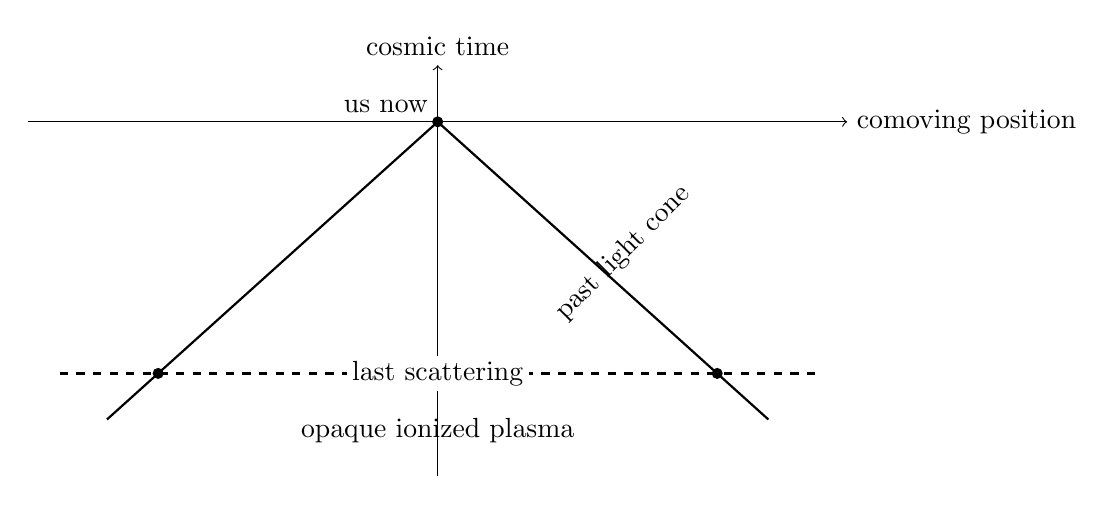
\begin{tikzpicture}[x=1.0cm,y=0.9cm]
\draw[->] (0,0)--(0,5.8) node[above] {cosmic time};
\draw[->] (-5.2,5.0)--(5.2,5.0) node[right] {comoving position};
\draw[thick] (0,5.0)--(-4.2,0.8);
\draw[thick] (0,5.0)--(4.2,0.8);
\draw[thick,dashed] (-4.8,1.45)--(4.8,1.45);
\fill (0,5.0) circle (2pt) node[above left] {us now};
\fill (-3.55,1.45) circle (2pt);
\fill (3.55,1.45) circle (2pt);
\node[fill=white,inner sep=2pt] at (0,1.45) {last scattering};
\node at (0,0.65) {opaque ionized plasma};
\node[rotate=45] at (2.35,3.15) {past light cone};
\end{tikzpicture}
\end{coursefitfigure}
\caption{Elektromagnetische Beobachtungen reichen entlang des vergangenen Lichtkegels nur bis zur Oberfläche der letzten Streuung zurück. Frühere Photonen wurden wiederholt am ionisierten Plasma gestreut.}
\label{fig:c07-last-scattering}
\end{figure}

\begin{classroomqa}
\audiencequestion{Beendet die Entkopplung jede Möglichkeit, frühere Epochen zu beobachten?}
\lecturerresponse{Sie beendet die direkte Beobachtung im elektromagnetischen Bereich, weil das Plasma für Photonen undurchsichtig war. Schwächer wechselwirkende Boten können früher entkommen: Fossile Neutrinos erlauben prinzipiell den Blick auf eine frühere Schicht, und Gravitationsstrahlung könnte Informationen aus noch früherer Zeit übermitteln. Unser Wissen über die Zeit vor der letzten Streuung ist also weitgehend indirekt, aber nicht beliebig. \lecturetimestamp{01:32:27--01:36:31}}
\end{classroomqa}

\begin{classroomqa}
\audiencequestion{Welchen absoluten Wert hatte \(a\) am Anfang, und war das Universum notwendigerweise ein winziges, endliches Objekt?}
\lecturerresponse{Im flachen Raum haben nur Verhältnisse von Skalenfaktoren eine invariante Bedeutung; die Normierung von \(a\) ist beliebig. Auch ein negativ gekrümmter räumlicher Schnitt kann unendlich sein. Ein geschlossenes Universum mit \(k=+1\) hat einen endlichen Krümmungsradius, doch Beobachtungen bestimmen weiterhin Expansionsverhältnisse und keine bekannte ursprüngliche Größe. Der heiße Urknall bedeutet für sich genommen nicht, dass der gesamte Raum eine winzige Kugel war. \lecturetimestamp{01:30:05--01:32:22}}
\end{classroomqa}

\begin{classroomqa}
\audiencequestion{Da die kosmische Mikrowellenhintergrundstrahlung älter ist als die Galaxien: Zeigt ihr Anblick uns, ob es heute jenseits unseres beobachtbaren Bereichs Galaxien gibt?}
\lecturerresponse{Nein. Die Hintergrundstrahlung zeigt eine weit entfernte Region so, wie sie bei der Entkopplung war, nicht so, wie sie heute ist. Das Licht heutiger Galaxien in hinreichend großer Entfernung hatte noch nicht genug Zeit, uns zu erreichen. Für die Annahme, dass es jenseits unseres Horizonts weiterhin Galaxienpopulationen gibt, sprechen die beobachtete großräumige Homogenität und das Fehlen eines sichtbaren Randes, nicht eine direkte Sicht, die uns die kosmische Mikrowellenhintergrundstrahlung verschafft. \lecturetimestamp{01:59:01--02:00:58}}
\end{classroomqa}

Die resultierende Zeitleiste führt von der Gegenwart rückwärts über die Galaxienbildung und Entkopplung bis zur Materie--Strahlungs-Gleichheit. Noch früher bedeutet ein kleinerer Skalenfaktor eine höhere Temperatur und das Auftreten neuer Teilchensorten.

\section{Materie--Strahlungs-Gleichheit}

Geht man über die Entkopplung hinaus zurück, erscheint ein weiterer Meilenstein. Nichtrelativistische Materie und Strahlung verdünnen sich unterschiedlich:
\begin{equation}
\rho_m\propto a^{-3},
\qquad
\rho_r\propto a^{-4},
\qquad
\frac{\rho_m}{\rho_r}\propto a.
\label{eq:c07-equality-scaling}
\end{equation}
Zu späten Zeiten dominiert Materie, doch bei hinreichend kleinem \(a\) dominiert zwangsläufig Strahlung. Entsprechend ändert sich das Expansionsgesetz vom Verhalten in der Materie-Ära \(a\propto t^{2/3}\) in Richtung des Verhaltens in der Strahlungs-Ära \(a\propto t^{1/2}\).

Eine bewusst grobe Abschätzung geht von \(10^8\) Photonen pro Proton, einer charakteristischen Energie der Photonen der kosmischen Mikrowellenhintergrundstrahlung von \(10^{-4}\,\mathrm{eV}\) und einer Ruheenergie des Protons von \(10^9\,\mathrm{eV}\) aus. Vernachlässigt man dunkle Materie, ergibt sich
\begin{equation}
\left(\frac{\rho_m}{\rho_r}\right)_0
\sim
\frac{10^9}{10^8\,10^{-4}}
\sim10^5.
\end{equation}
Dann wird die Abschätzung korrigiert: Dunkle Materie trägt wesentlich mehr Masse bei als leuchtende Baryonen, wodurch sich die gerundete Schätzung auf \(10^6\) erhöht. Mit dieser Rechnung legt Gleichung~\eqref{eq:c07-equality-scaling} den Zeitpunkt der Gleichheit fest als
\begin{equation}
\frac{a_{\rm eq}}{a_0}\sim10^{-6},
\qquad
\frac{T_{\rm eq}}{T_0}\sim10^6.
\label{eq:c07-equality-estimate}
\end{equation}
Dies sind grobe Abschätzungen zur Bestimmung der Skala für die Vorlesung, keine präzise Anpassung kosmologischer Parameter. Sie sollen zeigen, wie unterschiedliche Potenzen von \(a\) aufeinanderfolgende thermische Epochen festlegen.

Die strahlungsdominierte Epoche liegt hinter der elektromagnetischen Grenze der letzten Streuung. Ihre Existenz folgt jedoch aus den gemessenen Dichten der späten Epoche und den bekannten Skalierungsgesetzen. Bei hinreichend hoher Temperatur gilt schließlich die Annahme nicht mehr, dass die Anzahl der Protonen, Elektronen und Photonen jeweils für sich erhalten bleibt, denn energiereiche Stöße beginnen, massive Teilchen--Antiteilchen-Paare zu erzeugen.

\begin{classroomqa}
\audiencequestion{Gilt die Aussage, dass die Anzahl von Photonen und Protonen erhalten bleibt, auch für Sternenlicht und beliebig hohe Temperaturen?}
\lecturerresponse{Nein. Sie gilt für die fossile Population der kosmischen Mikrowellenhintergrundstrahlung in dem Zeitraum, in dem Reaktionen mit Änderung der Teilchenzahl unwirksam sind. Sternenlicht entstand später und ist für die Photonenzahl vernachlässigbar. Bei hinreichend hoher Temperatur verändert Paarerzeugung den Teilchenbestand, sodass die jeweilige Teilchenzahl nicht erhalten bleibt. Die Rekombination selbst fügt höchstens ungefähr ein Photon pro Elektron hinzu, also nur eines von \(10^8\) der vorhandenen Photonen der kosmischen Mikrowellenhintergrundstrahlung. \lecturetimestamp{01:26:24--01:27:40}}
\end{classroomqa}

\section{Paarerzeugung und die beinahe symmetrische Ursuppe}

Bei einer Temperatur in der Größenordnung
\begin{equation}
T\sim10^{10}\,\mathrm{K},
\qquad
\frac{a_0}{a}\sim10^{14},
\end{equation}
liegt die charakteristische Photonenenergie bei etwa einem Megaelektronenvolt und damit auf einer Skala vergleichbar mit der Ruheenergie, die zur Erzeugung eines Elektron--Positron-Paares benötigt wird. Dann können zwei Photonen über folgende Reaktion miteinander wechselwirken:
\begin{equation}
\gamma+\gamma
\longleftrightarrow
e^-+e^+.
\label{eq:c07-pair-reaction}
\end{equation}
Die genaue Schwelle hängt von der Stoßkinematik ab, doch die Ruheenergie des Elektrons, \(m_ec^2\), legt die maßgebliche Skala fest.

Paarerzeugung und Annihilation gleichen einander rasch aus. Sind zu wenige Paare vorhanden, füllen Photonenkollisionen ihren Bestand wieder auf; sind zu viele vorhanden, führt die Annihilation ihre Energie den Photonen zurück. Die Häufigkeiten von Photonen, Elektronen und Positronen werden daher durch die Temperatur bestimmt und sind im relativistischen Plasma alle von vergleichbarer Größenordnung. Ihre späteren Anzahlen lassen sich nicht mehr einfach aus den früheren ableiten.

\begin{classroomqa}
\audiencequestion{Wie kann dieses mit Paaren gefüllte Plasma elektrisch neutral bleiben, wenn es bereits Elektronen gibt, die zum Ladungsausgleich der Protonen benötigt werden?}
\lecturerresponse{Bei jeder Reaktion entsteht eine negative und eine positive Ladung, sodass die Paare keine Nettoladung hinzufügen. Sie bilden eine riesige, nahezu symmetrische Population, die einem winzigen Elektronenüberschuss überlagert ist. Die einzelnen Elektronen sind nicht unterscheidbar; nur die Differenz \(N_{e^-}-N_{e^+}\) erinnert an die Ladung, die zum Ausgleich der Protonen benötigt wird. \lecturetimestamp{01:42:31--01:43:14}}
\end{classroomqa}

Paarreaktionen verändern die Summe, erhalten aber die Differenz:
\begin{equation}
N_{e^-}+N_{e^+}\quad\hbox{changes},
\qquad
N_{e^-}-N_{e^+}=\hbox{constant}.
\label{eq:c07-pair-invariants}
\end{equation}
In der heißen Ursuppe ist \(N_{e^-}+N_{e^+}\) von derselben Größenordnung wie \(N_\gamma\), während der verbleibende Überschuss in der Größenordnung der viel kleineren Protonenzahl liegt. Das gerundete Verhältnis ist daher
\begin{equation}
\boxed{
\frac{N_{e^-}-N_{e^+}}
{N_{e^-}+N_{e^+}}
\sim10^{-8}
}.
\label{eq:c07-asymmetry}
\end{equation}
Auf jeweils \(10^8\) Elektron--Positron-Paare kam ungefähr ein überschüssiges Elektron.

Damit kehrt sich die ursprüngliche Frage um. Erstaunlich ist nicht einfach, dass es viele Photonen gibt. Bei hoher Temperatur treten Photonen und Paare natürlicherweise in vergleichbarer Häufigkeit auf. Das Rätsel ist, warum sich die Häufigkeiten negativer und positiver Teilchen überhaupt unterscheiden und warum ihr relativer Unterschied winzig statt genau null oder von der Größenordnung eins ist. Ein symmetrischer Anfangszustand und symmetrische Paarerzeugung ergäben keinen Überschuss. Der mikroskopische Ursprung der von null verschiedenen Asymmetrie ist das Problem, das wir im nächsten Abschnitt weiterverfolgen.

Bei Temperaturen, die um weitere zwei oder drei Größenordnungen höher liegen, lässt sich die Protonenstruktur nicht mehr vernachlässigen. Stöße erzeugen Quarks und Antiquarks, während Protonen sich in ihre Bestandteile auflösen; Photonen, Leptonen, Quarks, Antiquarks, Gluonen und alle leichten genug dunklen Teilchensorten bilden ein noch heißeres Plasma. Dort ist die Vakuumenergie dynamisch vernachlässigbar, weil die Strahlungsdichte wie \(a^{-4}\) zunimmt.

Der entsprechende Quarküberschuss ist durch die globale Ladungsneutralität an den Elektronenüberschuss gekoppelt. Drei Valenzquarks bilden ein Baryon, daher unterscheidet sich die Bilanzierung um konventionelle Faktoren; die verbliebene baryonische Materie und die verbliebenen Elektronen sind jedoch keine voneinander unabhängigen Ladungsungleichgewichte. Ihre gemeinsame geringe Häufigkeit ist ein Relikt des frühen Universums.

Verfolgen wir das Elektron--Positronenplasma wieder vorwärts. Sobald die Temperatur unter die Schwelle für die Paarerzeugung fällt, geht die Annihilation weiter, während die umgekehrte Reaktion selten wird. Fast jedes Elektron findet ein Positron, die Paarenergie wird zu Strahlung, und nur die winzige überschüssige Elektronenpopulation bleibt zurück. Die Materie um uns herum ist dieses verbleibende Ungleichgewicht, keine repräsentative Stichprobe aus der einst enormen Paarpopulation.

\begin{classroomqa}
\audiencequestion{Was geschah mit den Protonen während der Ära der Elektron--Positronen-Annihilation?}
\lecturerresponse{Zu diesem Zeitpunkt war die Temperatur hoch genug, um Elektronenpaare zu erzeugen, aber noch nicht hoch genug, um in großer Zahl Proton--Antiprotonen-Paare zu erzeugen oder Protonen in Quarks aufzulösen. Die Protonenpopulation war daher klein, blieb aber bestehen, und die Ladungsneutralität erforderte \(N_{e^-}-N_{e^+}\simeq N_p\). \lecturetimestamp{01:55:35--01:56:53}}
\end{classroomqa}

Das sichtbare Universum scheint überall dasselbe Vorzeichen des Materieüberschusses aufzuweisen. Als Beleg wird im Unterricht das Fehlen von Antikernen in der kosmischen Strahlung angeführt: Sekundärkollisionen können gelegentlich Antiprotonen erzeugen, doch von einer Antigalaxie wären komplexe Antikerne zu erwarten. Dies ist ein Beobachtungsargument aus der Zeit der Vorlesung und keine Behauptung, dass Regionen jenseits des beobachtbaren Horizonts untersucht worden seien.

\begin{classroomqa}
\audiencequestion{Könnte der beobachtete Materieüberschuss eine lokale Fluktuation sein, während es außerhalb unseres Sichtbereichs Regionen aus Antimaterie gibt?}
\lecturerresponse{Dasselbe Vorzeichen über das gewaltige beobachtbare Volumen hinweg ist viel zu gleichförmig, um eine zufällige Fluktuation zu sein. Es verlangt nach einer dynamischen Erklärung. Jenseits des beobachtbaren Bereichs fehlen jedoch direkte Belege; ein Übergang zu einem anderen Gebiet lässt sich nicht allein dadurch ausschließen, dass man über die Reichweite des Lichts hinausblickt. \lecturetimestamp{01:56:57--01:58:47}}
\end{classroomqa}

\begin{classroomqa}
\audiencequestion{Ist die Erklärung durch Materie--Antimaterie bereits eine präzise quantitative Theorie, und findet die Vereinheitlichung der Kräfte bei dieser Temperatur statt?}
\lecturerresponse{Es gibt eine qualitative Theorie dazu, wie eine kleine Asymmetrie entstehen kann, doch der gerundete Wert \(10^{-8}\) wird hier nicht aus einem eindeutigen mikroskopischen Modell hergeleitet. Die Vereinheitlichung der Kräfte gehört zu Temperaturen, die weit über denen der Epoche der Elektronenpaare liegen. Beide Fragen erfordern eine Physik, die über die hier behandelten thermischen Orientierungspunkte hinausgeht. \lecturetimestamp{01:51:36--01:52:24}}
\end{classroomqa}

\section{Was Sie mitnehmen sollten}

Die thermische Geschichte wird durch Reaktionsraten und Schwellenwerte bestimmt. Rasche Streuung sorgt für eine gemeinsame Temperatur; die Bildung neutraler Atome beseitigt die Streuzentren; und die gleichmäßige Expansion verschiebt anschließend das eingefrorene Planck-Spektrum zu längeren Wellenlängen, ohne seine Form zu zerstören. Die kosmische Mikrowellenhintergrundstrahlung ist daher zugleich ein Thermometer für die Strahlung und eine sichtbare Oberfläche, die das Ende des direkten elektromagnetischen Zugangs zum früheren Plasma markiert.

Der Photonenüberschuss macht die Rekombination zu einer Frage des hochenergetischen Spektralausläufers statt der mittleren Energie. Die Skala \(T_{\rm dec}/T_0\sim10^3\) kennzeichnet die letzte Streuung, während die unterschiedlichen Verdünnungsgesetze für Materie und Strahlung eine frühere Ära der Gleichheit kennzeichnen. Bei noch höheren Temperaturen löscht die Paarerzeugung die Erinnerung an die Gesamtzahlen von Elektronen und Positronen, bewahrt aber ihren winzigen Unterschied. Diese verbleibende Asymmetrie, die sich im baryonischen Sektor widerspiegelt, ist die unerklärte Anfangsbedingung, der sich die nächste Untersuchung stellen muss.